\section{Results}
\label{sec:results}
\subsection{Replacement changes temporal eligibility}
The source-derived challenge contains twenty accepted paragraphs from eighteen articles.
Its 45 claims have 33 directed replacement links.
Twenty-five links record consecutive replacements.
Eight links follow complete ordered succession lists.
Both source reviews check every accepted graph before certificate evaluation.
The frozen boundary schedule yields 73 point queries.

Both policies retain identical date bounds, explicit ends, and known source orders.
With five excerpts, replacement changes 34 contexts relative to interval overlap.
With one excerpt, omitting replacement marks 42 unstable contexts as stable.
Every unstable decision has two order-feasible timelines with different literal excerpts.
Table~\ref{tab:replacement} reports both budgets.
\begin{table}[t]
\centering
\small
\setlength{\tabcolsep}{5pt}
\begin{tabular}{rrrrr}
\toprule
$k$ & Queries & Changed & Missed & Stable \\
\midrule
1 & 73 & 33 & 42 & 25 \\
5 & 73 & 34 & 0 & 25 \\
\bottomrule
\end{tabular}
\caption{Source-derived replacement challenge. Changed counts possible contexts differing from interval control. Missed counts replacement-sensitive contexts that interval control marks stable. Stable counts certified contexts with replacement. Both policies enforce known source order.}
\label{tab:replacement}
\end{table}


Known order also sharpens the source decisions.
A Levadia passage places Bondarenko's appointment in 2001 and Rautiainen's succession in November 2001.
Enforcing their stated order resolves one additional stable query at each budget.
Under independent dates, the fast compiler matches all 388 exact support judgments.
Appendix~\ref{app:replacement} records sampling, reviewed annotations, query construction, and complete witness replay.

\subsection{Constraints resolve avoidable uncertainty}
Exhaustive world enumeration confirms all 100,800 support decisions and 30,240 fixed-ranking context decisions.
The oracle rejects all twenty inconsistent models.
Across the three predicates, constraints certify 929 contexts left unresolved by independent bounds.
These cases include overlapping lifetime bounds and uncertain event order.

For overlap queries, the hybrid first certifies 3,001 contexts without query-level constraint solving.
Selective solving recovers 312 additional stable contexts.
It returns two replayed timelines for each of the remaining 6,767 unstable contexts.
Table~\ref{tab:hybrid} compares it with a lazy exact solver using the same ranking and stopping rule.
The hybrid uses 59.79\% fewer exact claim queries and 55.67\% fewer feasibility calls.
These counts measure solver work after ranking.
\begin{table}[t]
\centering\small
\begin{tabular}{@{}rrrr@{}}
\toprule
Budget & Lazy exact & Hybrid & Saved (\%)\\
\midrule
1 & 4,361 & 1,645 & 62.28\\
3 & 12,019 & 4,849 & 59.66\\
5 & 16,800 & 6,849 & 59.23\\
\midrule
\textbf{All} & \textbf{33,180} & \textbf{13,343} & \textbf{59.79}\\
\bottomrule
\end{tabular}
\caption{Exact claim queries on 120 constrained models and 28 windows. Both methods stop after filling the possible context. Each budget covers 3,360 requests. Their contexts and stability decisions agree throughout.}
\label{tab:hybrid}
\end{table}


A separate grid tests 476 configurations with two distinct supplying witnesses.
The complete compiler matches all 13,328 claim--window decisions.
Each single-witness subset fails in every configuration.
Removing the forced-retirement witness wrongly includes 1,750 possible cases.
Removing the optional-retirement witness wrongly includes 5,576 guaranteed cases.


\subsection{Source coverage controls the automatic track}
Figure~\ref{fig:coverage} reports every evaluated question.
The automatic adapter reaches modeled contexts for 309 of 3,178 questions, or 9.72\%.
It finds 245 stable contexts and 64 unstable contexts within this group.
Stable means unchanged selected excerpts under the supplied date model.
The other questions yield 2,800 parsed all-fallback contexts and 69 unparsed windows.
Fallback eligibility stays fixed and contributes no temporal certificate.
\begin{figure}[t]
\centering
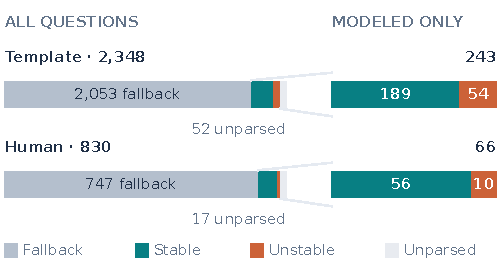
\includegraphics[width=\columnwidth]{figures/coverage.pdf}
\caption{Coverage before conditional stability. The left bars show every question. The right bars expand contexts containing modeled claims. Gray fallback excerpts have fixed eligibility. Stable and unstable counts apply only to the modeled subsets.}
\label{fig:coverage}
\end{figure}

The adapter models 493 development claims and 464 test claims.
They occupy 1.49\% and 1.36\% of indexed source units.
A model-assisted source audit accepts 54 of sixty event interpretations.
Grounding blocks both learned extraction pilots.
Two learned extraction variants return 87 records from six shared calibration paragraphs.
None passes both literal grounding and holder--date checks.
The deterministic adapter therefore requires explicit supporting spans before issuing a temporal certificate.
Appendix~\ref{app:pipeline} retains every source judgment and failed extraction output.

Independent replay verifies all 128 date assignments for the 64 unstable contexts.
Each pair changes the rendered source excerpts.
Forty-one exclusions use explicit retirement dates; twenty-three use late starts.
For example, a human question asks which title Peter Beattie held in February 1998.
The source dates his premiership from 1998 to 2007.
Starts on February 1 and December 31 produce different contexts while respecting that source precision.
The automatic track exercises these interval boundaries.

\subsection{Certificates compose with the relevance ranker}
The selected title-aware ranking reaches 67.61\% template span recall and 58.11\% human span recall.
Its gains over original BM25 with recency are 14.34 and 5.00 percentage points.
Their paired intervals are $[11.86,16.77]$ and $[0.69,9.10]$.
Adding recency to the selected ranker reaches 64.26\% human recall.
These gains belong to relevance ranking.
Possible support and the interval control select identical excerpts on the automatic track.
The appendix gives all ten matched retrieval rows.

Certificates also apply to all six prespecified ranking variants.
Every one of 18,654 query--ranking decisions matches full-mask selection.
Under the strongest human retrieval control, 102 of 120 modeled contexts remain stable.
With one excerpt, 90.9\% of template contexts and 97.0\% of human contexts are stable.
At twenty excerpts, these rates fall to 76.5\% and 78.8\%.
Each comparison retains the modeled cohort selected at $k=5$, so changing coverage cannot explain this decline.
A wider context can expose date-sensitive evidence that a narrow context excludes.
Table~\ref{tab:budget} reports intermediate budgets before word truncation.

\subsection{Answer sensitivity under structured decoding}
All 234 responses pass the unchanged parser, covering every primary and diagnostic condition.
Table~\ref{tab:reader_main} reports strict answer-set F1.
The title-aware ranking gains 11.11 points over original BM25 with recency, with interval $[3.33,19.44]$.
This difference follows the relevance ranking.
Possible and guaranteed support share every primary context and produce identical answers.
\begin{table}[t]
\centering\small
\begin{tabular}{@{}lrr@{}}
\toprule
Method & Primary & Diagnostic\\
\midrule
Original + year & 25.00 & 18.18\\
Title-aware & 36.11 & 9.09\\
Title-aware + year & 33.33 & 24.24\\
Possible support & 36.11 & 9.09\\
Guaranteed support & 36.11 & 18.18\\
\bottomrule
\end{tabular}
\caption{Strict answer-set F1 (\%). Temporal policies use title-aware BM25 without the year bonus.}
\label{tab:reader_main}
\end{table}


Seven diagnostic questions have different possible and guaranteed contexts.
Four produce different answer sets.
Guaranteed support gains 9.09 F1 points, with interval $[0.00,30.00]$.
Partial strict matches now separate F1 from exact match.
Appendix~\ref{app:reader} gives cardinality strata, every changed answer, and the complete decoding comparison.

